\documentclass[14pt]{extbook}
\usepackage{multicol, enumerate, enumitem, hyperref, color, soul, setspace, parskip, fancyhdr} %General Packages
\usepackage{amssymb, amsthm, amsmath, latexsym, units, mathtools} %Math Packages
\everymath{\displaystyle} %All math in Display Style
% Packages with additional options
\usepackage[headsep=0.5cm,headheight=12pt, left=1 in,right= 1 in,top= 1 in,bottom= 1 in]{geometry}
\usepackage[usenames,dvipsnames]{xcolor}
\usepackage{dashrule}  % Package to use the command below to create lines between items
\newcommand{\litem}[1]{\item#1\hspace*{-1cm}\rule{\textwidth}{0.4pt}}
\pagestyle{fancy}
\lhead{Progress Quiz 9}
\chead{}
\rhead{Version B}
\lfoot{9541-5764}
\cfoot{}
\rfoot{Summer C 2021}
\begin{document}

\begin{enumerate}
\litem{
Solve the rational equation below. Then, choose the interval(s) that the solution(s) belongs to.\[ \frac{4}{7x -5} + 3 = \frac{-3}{42x -30} \]\begin{enumerate}[label=\Alph*.]
\item \( x_1 \in [0.18, 0.4] \text{ and } x_2 \in [-0.5,2.5] \)
\item \( x \in [-1.11,-0.8] \)
\item \( \text{All solutions lead to invalid or complex values in the equation.} \)
\item \( x_1 \in [-1.11, -0.8] \text{ and } x_2 \in [-0.5,2.5] \)
\item \( x \in [-1.5,1.5] \)

\end{enumerate} }
\litem{
Choose the graph of the equation below.\[ f(x) = \frac{1}{(x + 3)^2} - 3 \]\begin{enumerate}[label=\Alph*.]
\begin{multicols}{2}\item 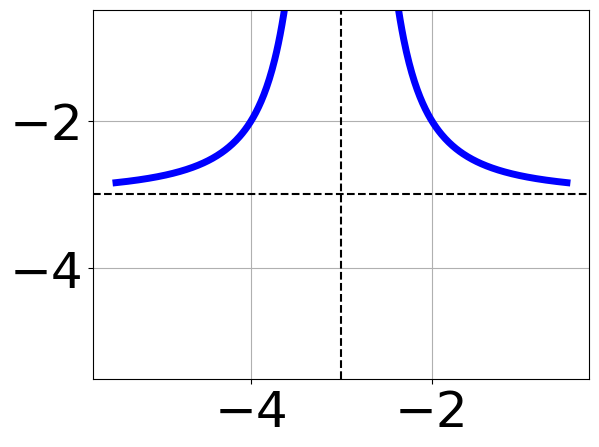
\includegraphics[width = 0.3\textwidth]{../Figures/rationalEquationToGraphCopyAB.png}\item 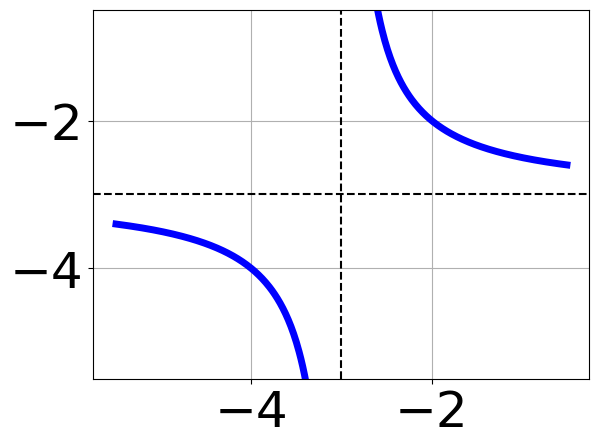
\includegraphics[width = 0.3\textwidth]{../Figures/rationalEquationToGraphCopyBB.png}\item 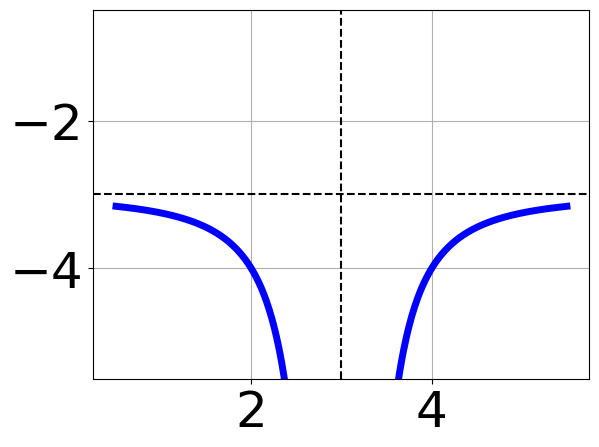
\includegraphics[width = 0.3\textwidth]{../Figures/rationalEquationToGraphCopyCB.png}\item 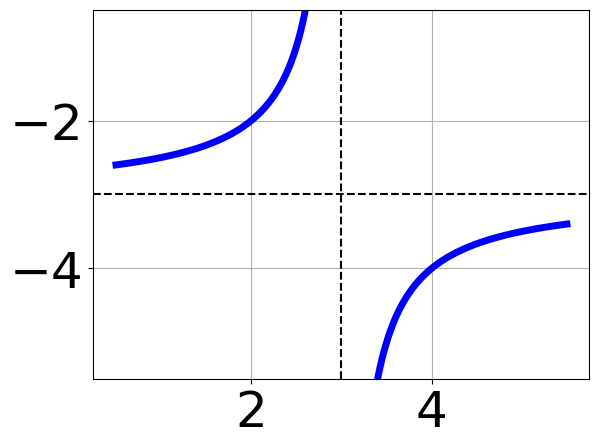
\includegraphics[width = 0.3\textwidth]{../Figures/rationalEquationToGraphCopyDB.png}\end{multicols}\item None of the above.
\end{enumerate} }
\litem{
Solve the rational equation below. Then, choose the interval(s) that the solution(s) belongs to.\[ \frac{3x}{-2x + 6} + \frac{-4x^{2}}{-8x^{2} +28 x -12} = \frac{-4}{4x -2} \]\begin{enumerate}[label=\Alph*.]
\item \( x_1 \in [-1.06, -0.31] \text{ and } x_2 \in [1.54,2.91] \)
\item \( \text{All solutions lead to invalid or complex values in the equation.} \)
\item \( x_1 \in [2.69, 3.2] \text{ and } x_2 \in [0.49,1.23] \)
\item \( x \in [0.38,1.49] \)
\item \( x \in [2.69,3.2] \)

\end{enumerate} }
\litem{
Determine the domain of the function below.\[ f(x) = \frac{5}{12x^{2} +2 x -24} \]\begin{enumerate}[label=\Alph*.]
\item \( \text{All Real numbers except } x = a, \text{ where } a \in [-1.5, -0.5] \)
\item \( \text{All Real numbers except } x = a, \text{ where } a \in [-24, -20] \)
\item \( \text{All Real numbers except } x = a \text{ and } x = b, \text{ where } a \in [-1.5, -0.5] \text{ and } b \in [-0.67, 2.33] \)
\item \( \text{All Real numbers except } x = a \text{ and } x = b, \text{ where } a \in [-24, -20] \text{ and } b \in [11, 13] \)
\item \( \text{All Real numbers.} \)

\end{enumerate} }
\litem{
Solve the rational equation below. Then, choose the interval(s) that the solution(s) belongs to.\[ \frac{-4}{-6x -5} + -8 = \frac{5}{-12x -10} \]\begin{enumerate}[label=\Alph*.]
\item \( x_1 \in [-0.7, 0.3] \text{ and } x_2 \in [-0.03,2.97] \)
\item \( x_1 \in [-0.7, 0.3] \text{ and } x_2 \in [-0.65,0.35] \)
\item \( \text{All solutions lead to invalid or complex values in the equation.} \)
\item \( x \in [-0.03,3.97] \)
\item \( x \in [-0.7,0.3] \)

\end{enumerate} }
\litem{
Choose the equation of the function graphed below.
\begin{center}
    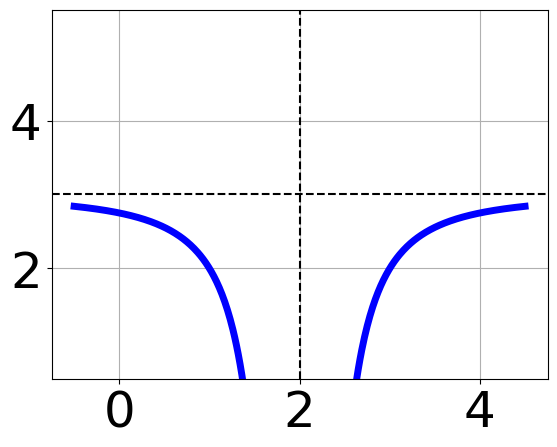
\includegraphics[width=0.5\textwidth]{../Figures/rationalGraphToEquationB.png}
\end{center}
\begin{enumerate}[label=\Alph*.]
\item \( f(x) = \frac{-1}{x - 2} + 3 \)
\item \( f(x) = \frac{1}{(x + 2)^2} + 3 \)
\item \( f(x) = \frac{-1}{(x - 2)^2} + 3 \)
\item \( f(x) = \frac{1}{x + 2} + 3 \)
\item \( \text{None of the above} \)

\end{enumerate} }
\litem{
Solve the rational equation below. Then, choose the interval(s) that the solution(s) belongs to.\[ \frac{-2x}{-4x -4} + \frac{-4x^{2}}{-20x^{2} -12 x + 8} = \frac{5}{5x -2} \]\begin{enumerate}[label=\Alph*.]
\item \( x \in [-0.13,0.5] \)
\item \( \text{All solutions lead to invalid or complex values in the equation.} \)
\item \( x_1 \in [-0.87, -0.46] \text{ and } x_2 \in [-3.5,-0.9] \)
\item \( x_1 \in [-0.87, -0.46] \text{ and } x_2 \in [1.8,3.3] \)
\item \( x \in [2.16,3.28] \)

\end{enumerate} }
\litem{
Choose the graph of the equation below.\[ f(x) = \frac{-1}{x + 1} + 3 \]\begin{enumerate}[label=\Alph*.]
\begin{multicols}{2}\item 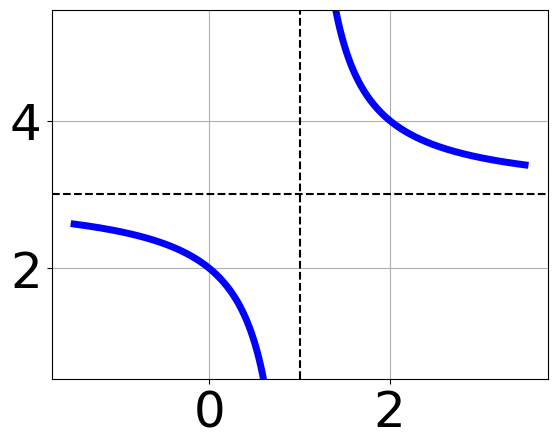
\includegraphics[width = 0.3\textwidth]{../Figures/rationalEquationToGraphAB.png}\item 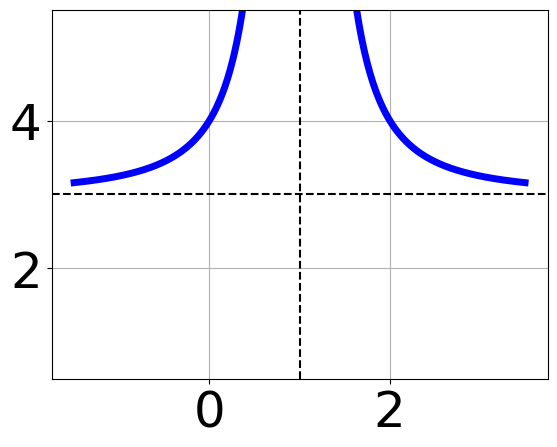
\includegraphics[width = 0.3\textwidth]{../Figures/rationalEquationToGraphBB.png}\item 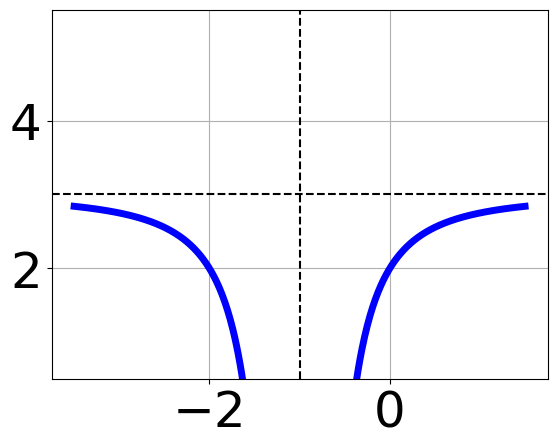
\includegraphics[width = 0.3\textwidth]{../Figures/rationalEquationToGraphCB.png}\item 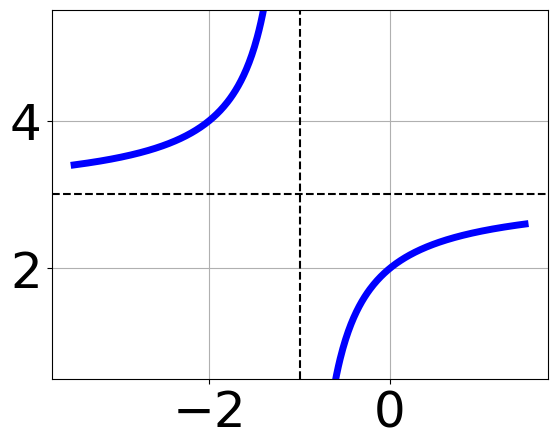
\includegraphics[width = 0.3\textwidth]{../Figures/rationalEquationToGraphDB.png}\end{multicols}\item None of the above.
\end{enumerate} }
\litem{
Choose the equation of the function graphed below.
\begin{center}
    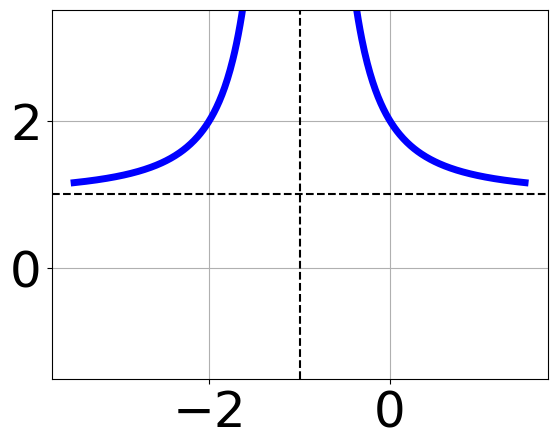
\includegraphics[width=0.5\textwidth]{../Figures/rationalGraphToEquationCopyB.png}
\end{center}
\begin{enumerate}[label=\Alph*.]
\item \( f(x) = \frac{1}{(x + 1)^2} + 1 \)
\item \( f(x) = \frac{1}{x + 1} + 1 \)
\item \( f(x) = \frac{-1}{x - 1} + 1 \)
\item \( f(x) = \frac{-1}{(x - 1)^2} + 1 \)
\item \( \text{None of the above} \)

\end{enumerate} }
\litem{
Determine the domain of the function below.\[ f(x) = \frac{6}{9x^{2} -25} \]\begin{enumerate}[label=\Alph*.]
\item \( \text{All Real numbers except } x = a, \text{ where } a \in [-4.67, 1.33] \)
\item \( \text{All Real numbers.} \)
\item \( \text{All Real numbers except } x = a \text{ and } x = b, \text{ where } a \in [-4.67, 1.33] \text{ and } b \in [-0.33, 3.67] \)
\item \( \text{All Real numbers except } x = a \text{ and } x = b, \text{ where } a \in [-16, -11] \text{ and } b \in [15, 20] \)
\item \( \text{All Real numbers except } x = a, \text{ where } a \in [-16, -11] \)

\end{enumerate} }
\end{enumerate}

\end{document}